% !TEX program = xelatex
\documentclass[12pt, a4paper]{article}

\usepackage{fontspec}
\setmainfont[Ligatures=TeX]{Linux Libertine O}

\usepackage[hidelinks, colorlinks = true, urlcolor = blue]{hyperref}
\usepackage{indentfirst}
\usepackage{graphicx}
\usepackage[left=0.5cm,right=0.5cm,top=0.2cm,bottom=0.2cm]{geometry}
\usepackage{lipsum}
\usepackage{caption}
\usepackage{subcaption}
\usepackage{dirtytalk}
\usepackage{xcolor}
\usepackage{wrapfig}

\usepackage{listings}
\usepackage{xparse}
\NewDocumentCommand{\codeword}{v}{%
\texttt{\textcolor{black}{#1}}%
}

\lstset{language=C,keywordstyle={\bfseries \color{black}}}\usepackage{titlesec}
\titlespacing{\section}{0pc}{1.5ex plus .1ex minus .2ex}{0pc}

%\setlength{\parindent}{1em}
%\setlength{\parskip}{1em}\title{Εργασία Στατιστικής}

\title{\textbf{Parallel and Distributed Systems \\ Parallel k-Nearest Neighbors}}
\author{Θεόδωρος Κατζάλης \\ ΑΕΜ:9282 \\ katzalis@auth.gr}
\date{13/1/2020}

\begin{document}

\sloppy
%\input{titlepage}
\maketitle


%\pagebreak

\section{Introduction}

The implementation of the task to find the k-Nearest Neighbors of a given dataset with N data points for all the points, is divided to three versions. The metric space is euclidean and the nearness is determined by the \textbf{euclidean distance}. It should be noted that one of the kth is assumed to be the point itself to be tested. So searching for k+1 neighbors is equivalent with searching for k excluding the self-point.

The first version (v0) is the serial one and the base for the next. For a query set of M points, it a) calculates the euclidean distance matrix $MxN$ and b) selects for each query point (per row) the k smaller values. For large matrices we block the query, but we assume that all the corpus points fit to memory. In other words, the $MxN$ distance matrix is sliced by blocks of rows, assuming that each block can have access to all the columns. 

In the second version (v1) \textbf{MPI} is introduced. Basically, we use v0 for each process, dividing the work in a balanced way. To make it clear, in this version we don't assume that each process can have full access to the data points of corpus (the N columns of the distance matrix). Instead each process take a slice $N_i$ of the initial corpus. This approach is mandatory because we assume that we don't have memory for all the N points. This is radically different than the blocking of v0 (per query) and now the \textbf{merging overhead} is introduced. The k neighbors calculated by each process isn't independent from the others (disrupted full view of N points) so we need each time to merge the results of the processes.

The last version (v2) introduces the vantage point tree as a more efficient data structure for an optimised v1. The goal is to reduce the number of neighbors needs to be assessed to find the nearest ones. But as we will see later this comes with quite a lot of cost and drawbacks at least for our implementation.

One of the biggest challenges needs to be addressed working with the above MPI versions (v1 and v2) is the \textbf{memory layout} of the data structure. It is preferred to use contiguous blocks of memory in order to be transferable. Otherwise, for more complicated data structures, a detailed memory layout needs to be stated clearly when using MPI routines and this is quite troublesome for some cases. For example offset and padding of memory when using \codeword{struct} in C should be considered. Usage of \textbf{nested vectors or tuples in C++} is probably not the best solution.  

Another challenge is the type of the \textbf{communication}. There are at least two approaches: 1) \textbf{Master-slave} technique\footnote{In the MPI implementations we assume that one process is able to have a full view of the corpus set so it can scatter chunks of data points to all the other processes}. The master process each time scatters the data to the rest of the processes. 2) Moving data in a \textbf{ring}, in which all nodes have sending and receiving roles.
Each of the above two types of communication can also divided to the usage of blocking or non blocking MPI routines. We preferred the non-blocking, asynchronous way to reduce as much as possible the communication cost. Start sending and receiving while computing.


\subsection{Versions implementation}

Calculating the distance matrix is fundamental for all the versions. For that purpose to speed up the process we use \textbf{cblas} routines that will play a very important role in the performance analysis because the acceleration is very dependent of the size of the matrix. The function \codeword{euclidean_distance_matrix()} serves that purpose.

Another important function all the versions use extensively is the \codeword{quickselect()}. The concept is to select the k smallest distances, so sorting isn't mandatory and needs to be avoided for better results. Our \codeword{quickselect()} is naive and takes as pivot the rightmost element. We didn't take into account a more delicate approach including medians of medians to address worst case performance. There is a lot of room for improvement for this. Another very good candidate is C++ utility \codeword{std::nth_element}. We sticked to the naive approach because with a slight code modification during the select, we swapped also the indices along with the values (distances in our case). 

For MPI communication, first in the master process we read the datasets, broadcast the n (number of points) and d (dimensions). Then each process calculates the size and the displacement memory of each data to be sent from the master. That way all the processes know how the data will be cycled later in the data-ring exchange. For the v1, the data to be sent is a subset of the corpus points and for the v2 the vantage point tree. \textbf{Vp-tree increased the complexity of communication} especially if nested structures are used for tree-representation. The requirement of contiguous memory blocks (serialization) forced us to use three simple arrays: the corpus, the indices and the vantage point coordinates in a \textbf{level order format}. We used \codeword{Isendv()} and \codeword{Irecv} routines for both versions (for v1 we tested also the master-slave technique using \codeword{Scatterv()} and \codeword{Gatherv()}. More here put ref). After each process finished its job, it compares the previous k-NN result with the current one, selecting again the k smallest (\codeword{quickselect()}).

For the \textbf{vp-tree} specifically instead of sending the subcorpus to each process and then calculate the tree, we create the tree only once per process in the start and then we pass it hand in hand to the other processes. To \textbf{make such a tree}, there are again two crucial steps. Calculate a) point to local corpus distance and b) find the median to later subdivide the corpus accordingly. Again we use \codeword{quickselect()} for the second but we decided not to use the already implemented \codeword{euclidean_distance_matrix()} for the first because cblas routines didn't accelerate the process (calculate point to points instead of multiple points to points). 

For \textbf{searching the tree}, another crucial operation, we chose C++ to help us a little bit and used \codeword{std::priority_queue}. That way we can keep track of the furthest distance (tau) while inserting new vantage points as neighbors candidates.

For the vp-tree we tried to add also the features of carefully selecting the vantage point and stop creating the tree sooner (more on this here put ref).

%For v1 and v2, left-rotate the calculated the size and the memory displacement. Since each process send its data to the next and receive from the previous, we use two lightweight routines, \codeword{left_rotate()} and \codeword{adjust_indeces()} to give the general view required to each process to keep track the correct indices of the global corpus set.

\section{Performance data}

Each dataset contains three performance graphs. For the first, we calculate the average time execution for k = 10, 40, 70, 100, for each set of processes. For the second and the third we test the effect of k for each version per set of processes. 
\begin{figure}[h!]
     \begin{subfigure}[b]{0.33\textwidth}
         \centering
         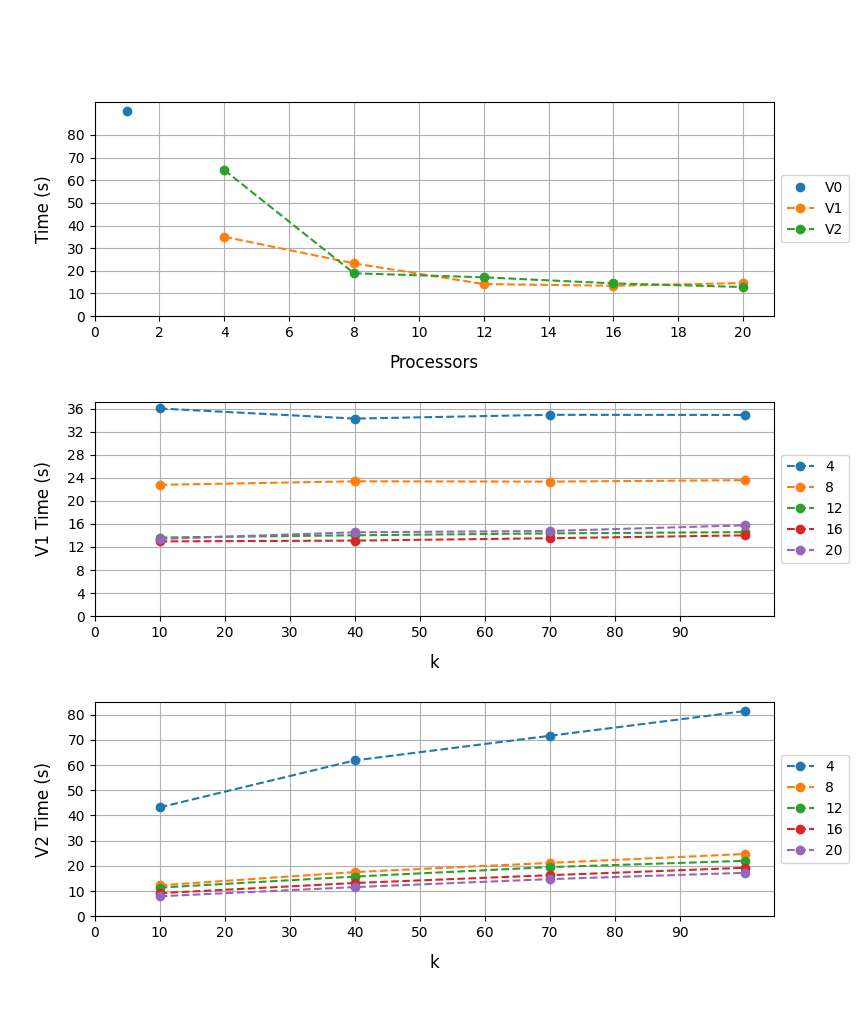
\includegraphics[height=.20\textheight, width=\textwidth, keepaspectratio]{assets/corel/histo.png}
    \caption{ColorHistogram n = 68.040 d = 32}
     \end{subfigure}
     \hfill
     \begin{subfigure}[b]{0.33\textwidth}
         \centering
         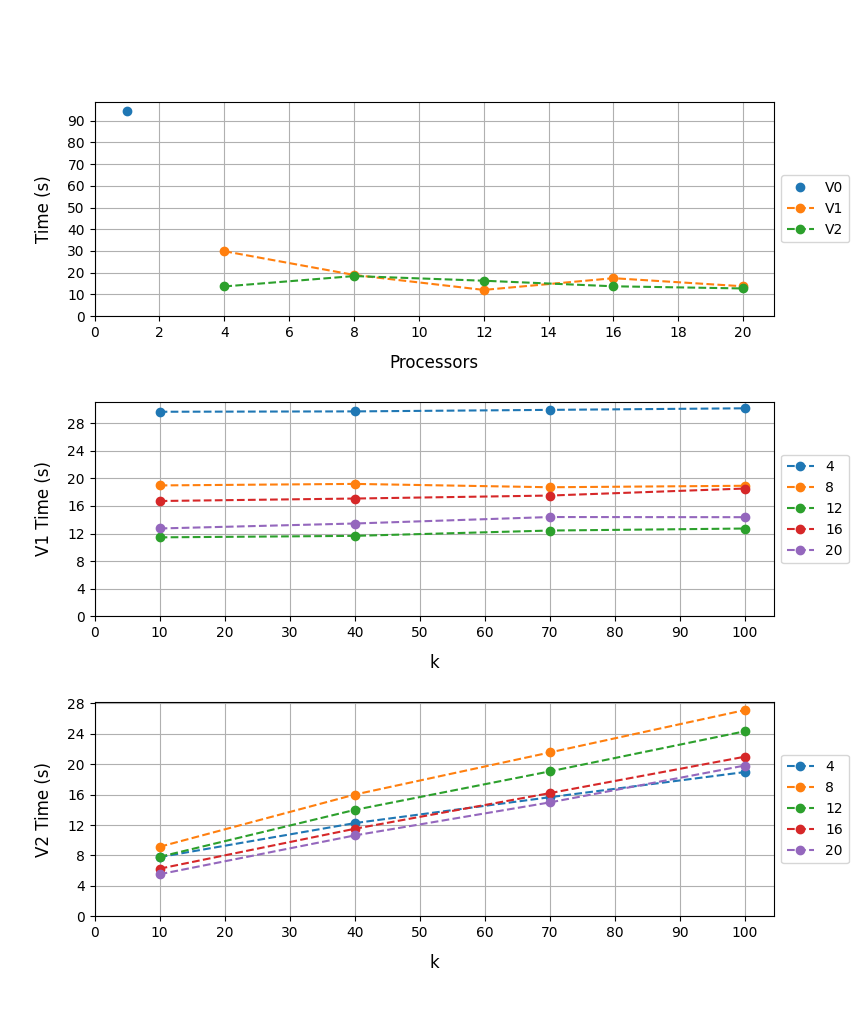
\includegraphics[height=.20\textheight, width=\textwidth, keepaspectratio]{assets/corel/moments.png}
         \caption{ColorMoments n = 68.040 d = 9}
     \end{subfigure}
     \begin{subfigure}[b]{0.33\textwidth}
         \centering
         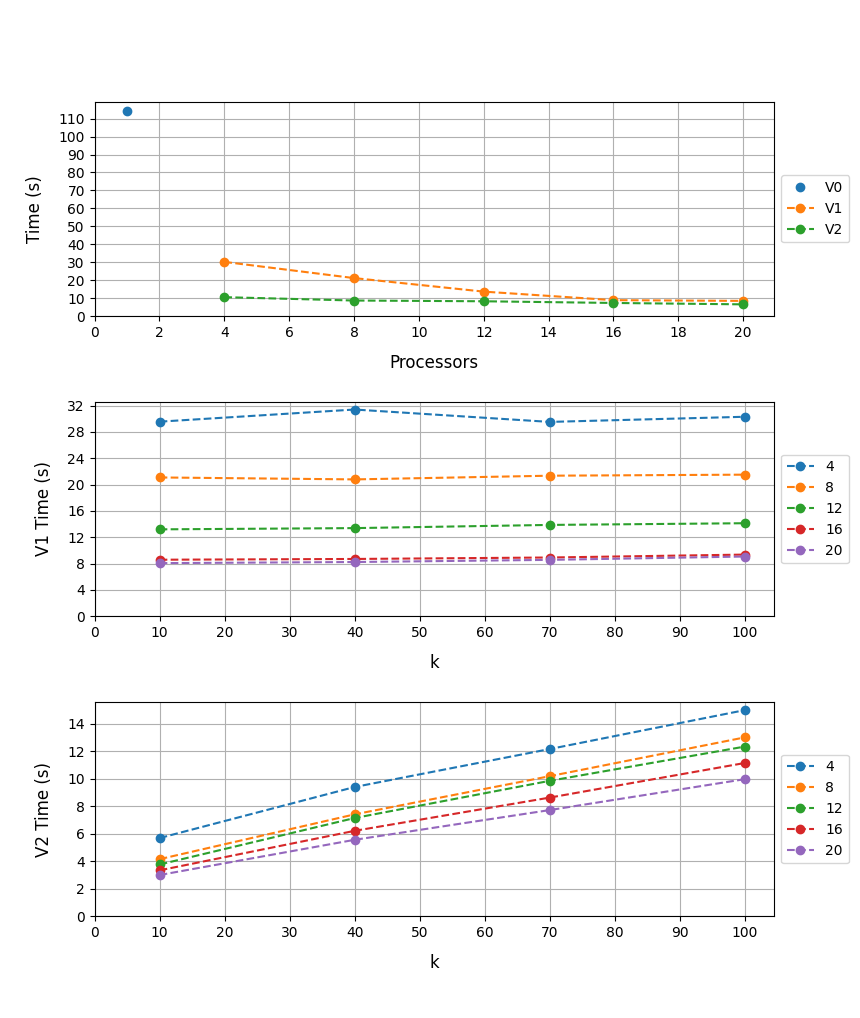
\includegraphics[height=.20\textheight, width=\textwidth, keepaspectratio]{assets/corel/texture.png}
         \caption{CoocTexture n = 68.040 d = 16} 
     \end{subfigure}
\end{figure}


\begin{figure}[h!]
     \begin{subfigure}[b]{0.33\textwidth}
         \centering
         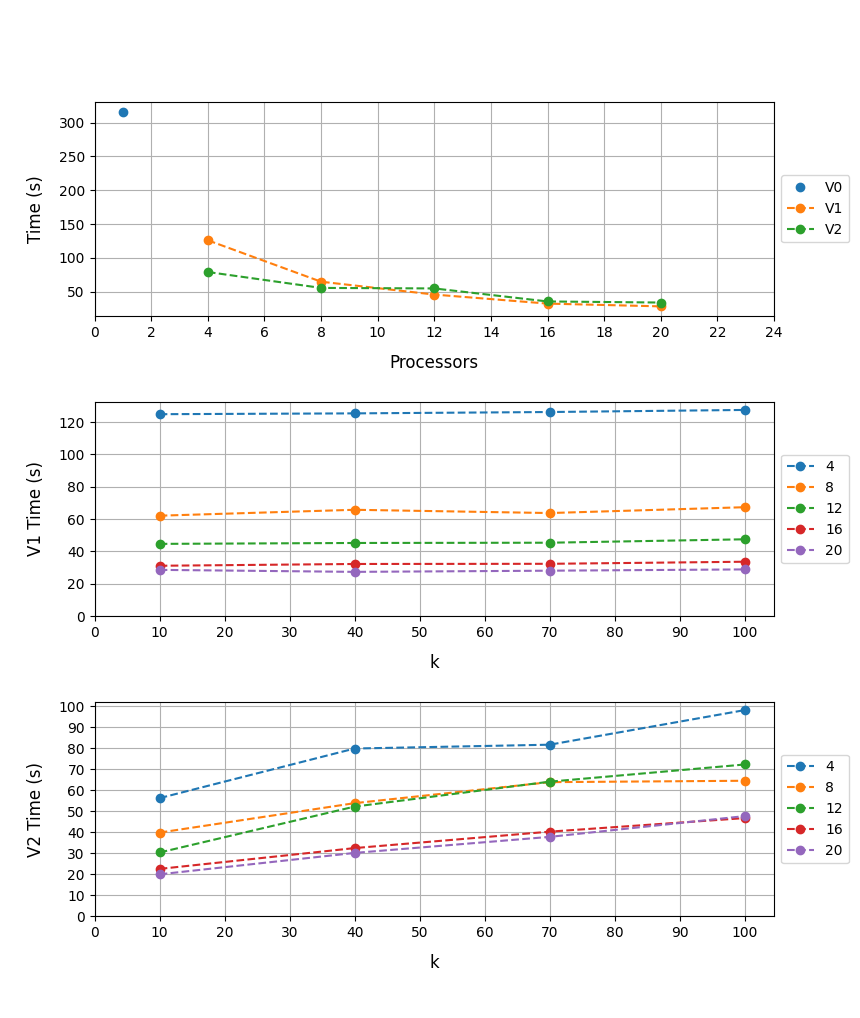
\includegraphics[height=.20\textheight, width=\textwidth, keepaspectratio]{assets/mini.png}
    \caption{MiniBooNE n = 130.064 d = 50}
     \end{subfigure}
     \hfill
     \begin{subfigure}[b]{0.33\textwidth}
         \centering
    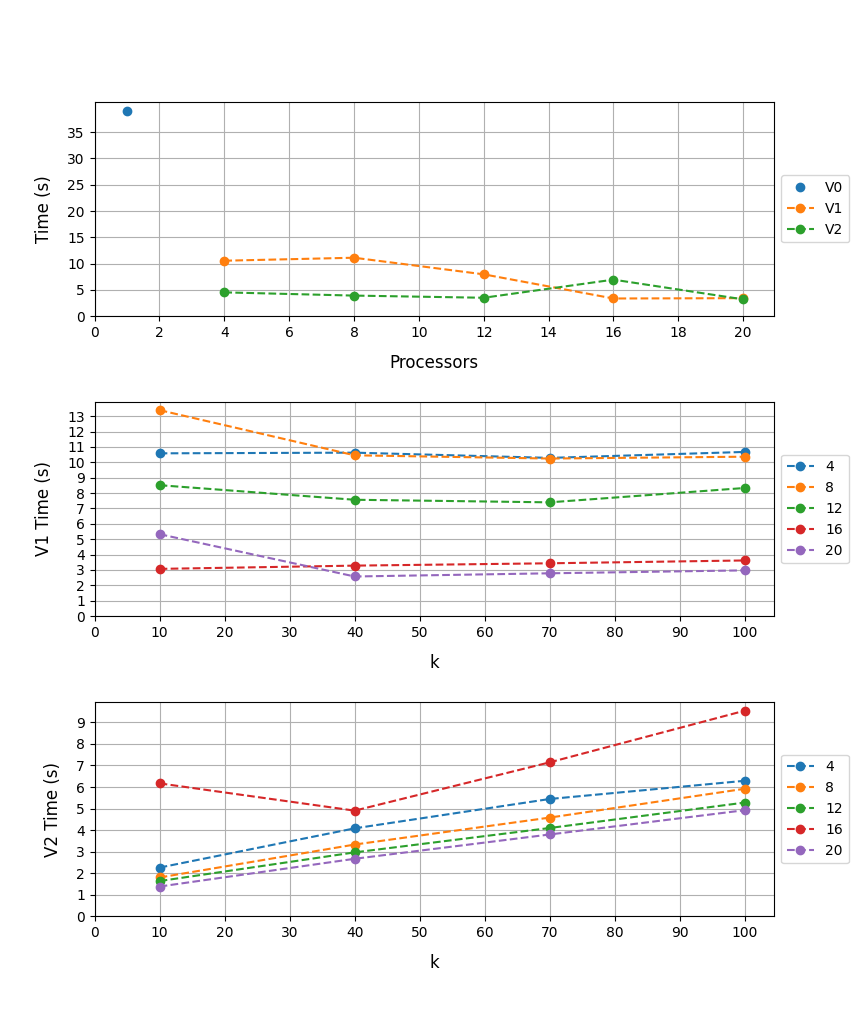
\includegraphics[height=.20\textheight, width=\textwidth, keepaspectratio]{assets/tv/timesnow.png}
         \caption{TV/TIMESNOW n = 39.252 d = 17}
     \end{subfigure}
     \begin{subfigure}[b]{0.33\textwidth}
         \centering
         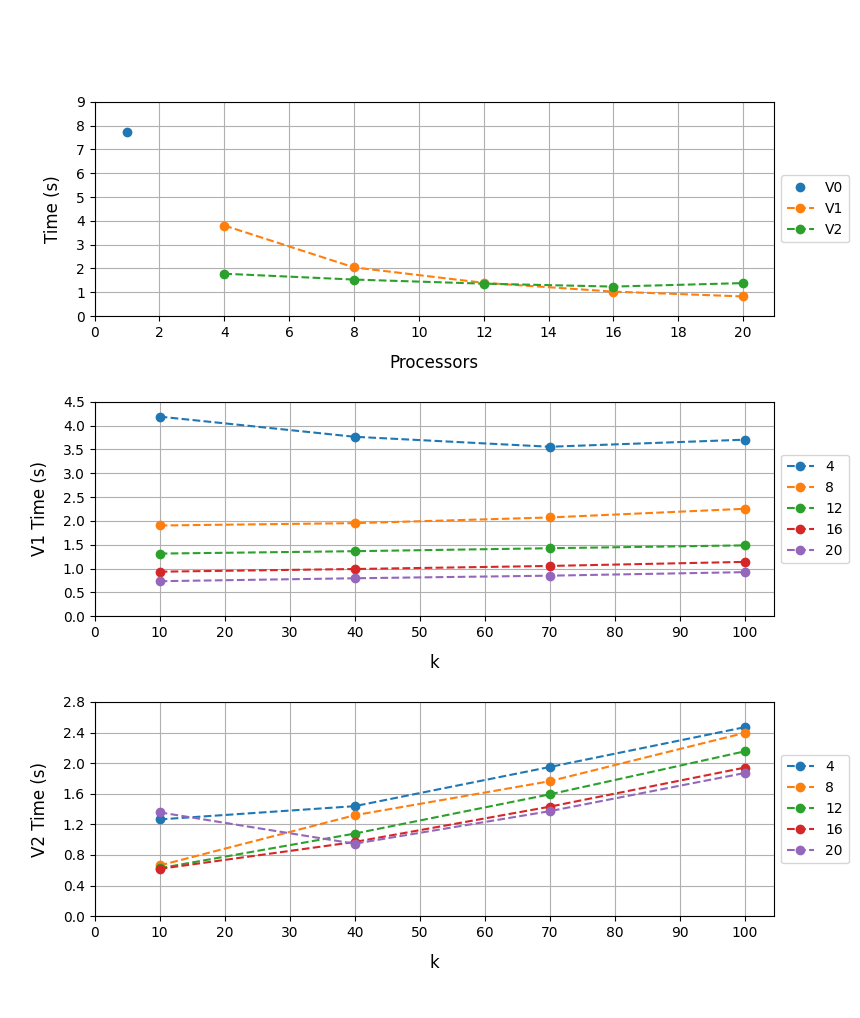
\includegraphics[height=.20\textheight, width=\textwidth, keepaspectratio]{assets/tv/bbc.png}
         \caption{TV/BBC n = 17.720 d = 17} 
     \end{subfigure}
\end{figure}


\begin{figure}[h!]
     \begin{subfigure}[b]{0.33\textwidth}
         \centering
         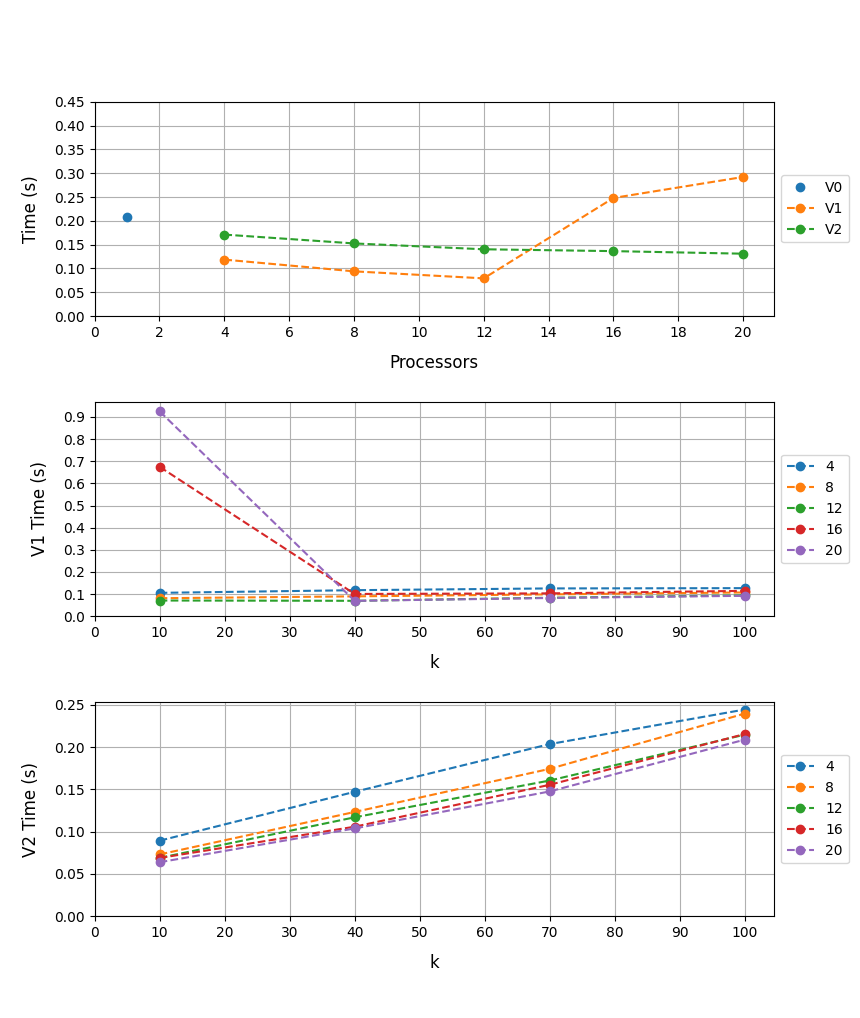
\includegraphics[height=.20\textheight, width=\textwidth, keepaspectratio]{assets/tv/cnnibn.png}
    \caption{TV/CNNIBN n = 3.317 d = 17}
     \end{subfigure}
     \hfill
     \begin{subfigure}[b]{0.33\textwidth}
         \centering
         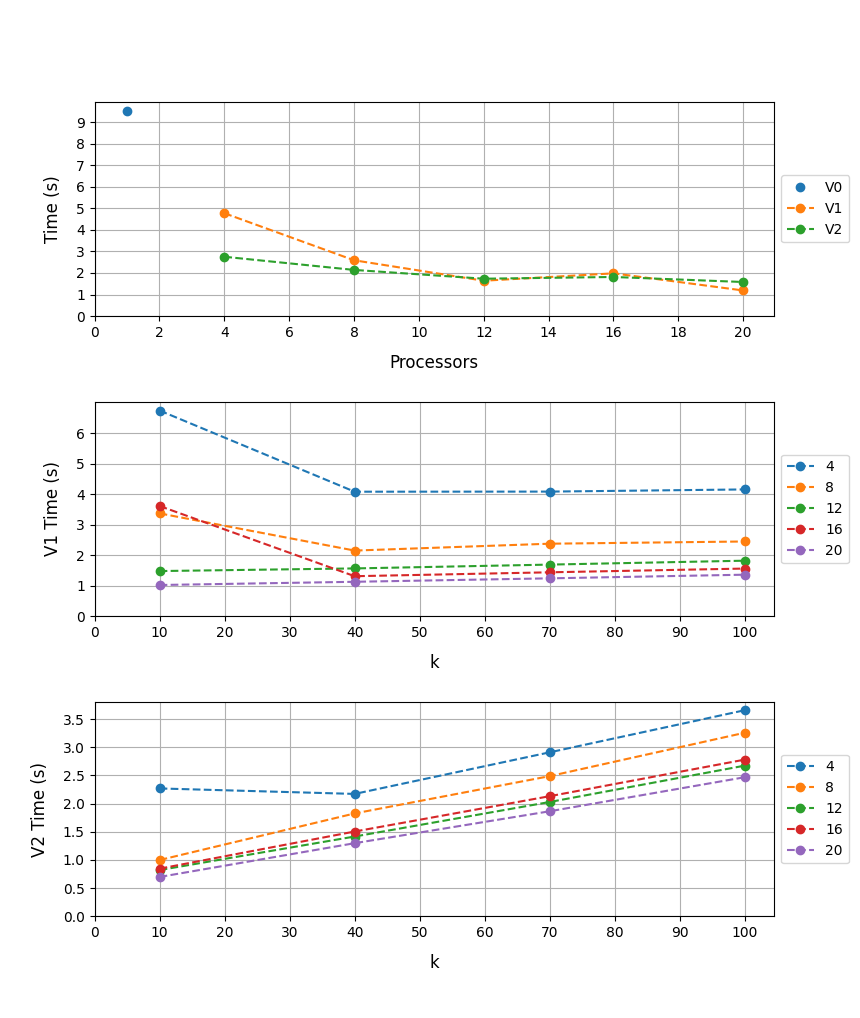
\includegraphics[height=.20\textheight, width=\textwidth, keepaspectratio]{assets/tv/cnn.png}
         \caption{TV/CNN n = 22.545 d = 17}
     \end{subfigure}
     \begin{subfigure}[b]{0.33\textwidth}
         \centering
         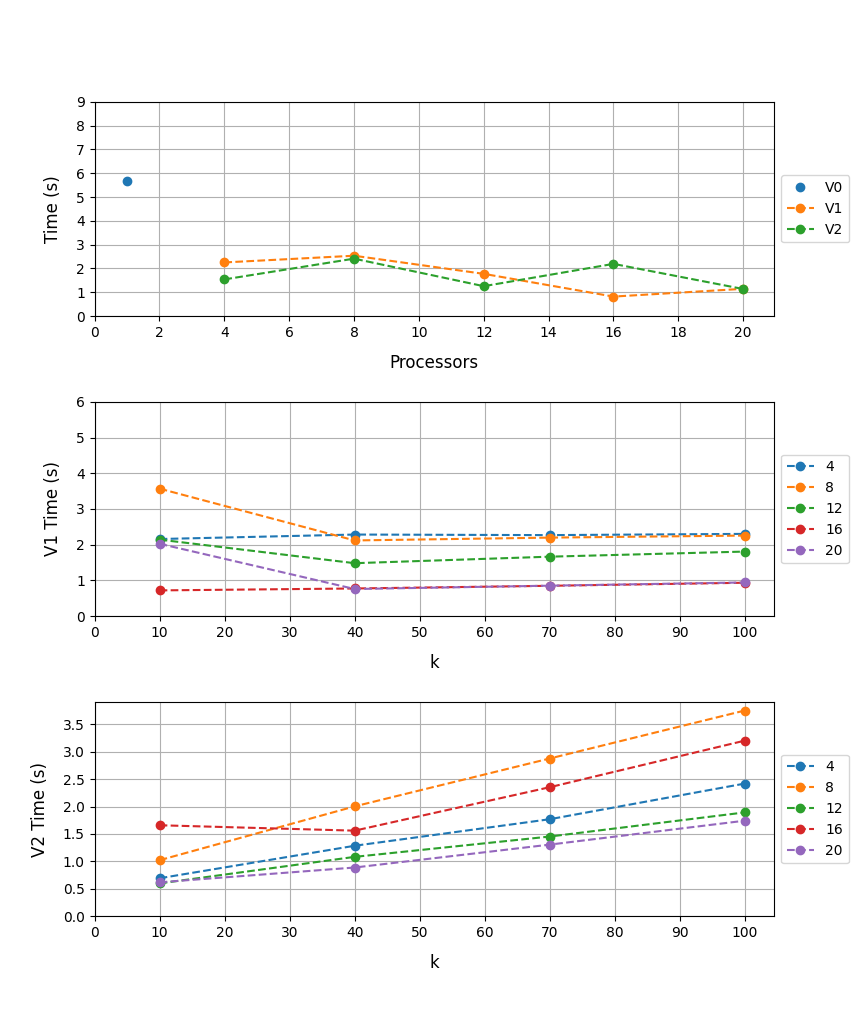
\includegraphics[height=.20\textheight, width=\textwidth, keepaspectratio]{assets/tv/ndtv.png}
         \caption{TV/NDTV n = 17.051 d = 17} 
     \end{subfigure}
\end{figure}

\pagebreak

\subsection{Conclusions}

\begin{itemize}
\itemsep-0.2em 
\item For a small number of neighbors (k) and dimensions (d), v2 outperforms v1 (ColorMoments, CoocTexture and TV/*). It should be emphasized that the aforementioned speedup is only limited to these specific conditions. 
    \item Poor scaling of v2 with respect to the number of neighbors (k) in contrast with v1 that its performance is almost constant.
    \item Poor scaling of v2 with respect to the number of dimensions (d).
    \item Speedup with respect to processes, isn't very clear. In some datasets we get constant speedup and in some others the time execution is barely improved as processes increase. We could claim that this is reasonable. One of the primary motives of using MPI is to be able to fit in memory the data rather than to speed up the processes. In our implementation each process isn't independent from the others. More processes means more updates and maybe the chunk size given to each data point may affect the performance of the cblas and the vptree search. So the result of the advantages and disadvantages are summed and produced the above results.

        Less processes may perform better for v1 because it is highly dependent of the size of the slices and how cblas accelerates for a given data chunk. In a general view, more processes improve performance. Increasing the numbers, decrease the size of the slices and the size of the tree or the subcorpus respectively and introduce more updates. The result is the outcome of the aforementioned advantages and disadvantages.
\end{itemize}

\begin{wrapfigure}[16]{r}{0.3\textwidth}
    \centering
    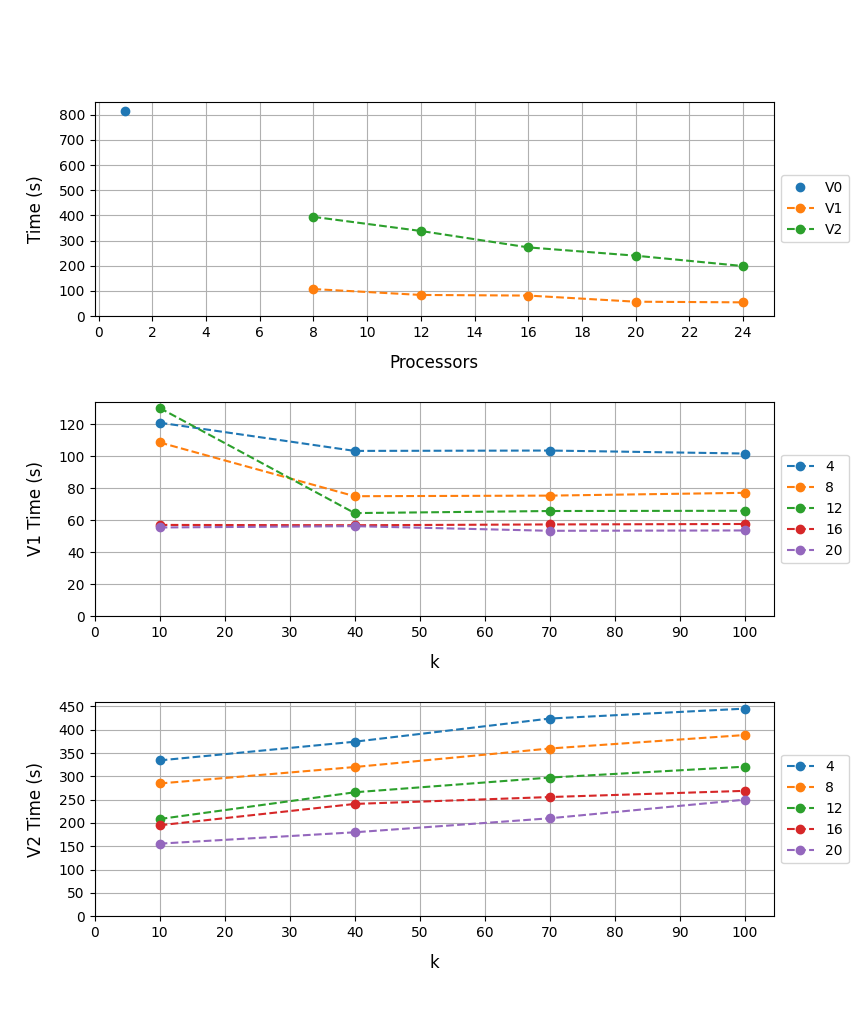
\includegraphics[height=.2\textheight, width=0.5\textwidth, keepaspectratio]{assets/black_sheep.png}
    \caption{features.csv \newline n = 106.574 d = 517}
\end{wrapfigure}

And now the last for the worst! In order to validate what we claimed regarding poor performance of v2, the features.csv dataset is a great candidate. As we can observe, the v2 performance is indeed terrible. It is 4 times slower than the v1. Of course the current implementation due to these results needs probably quite a lot of tuning to fix these performance deal-brakers. But we can state some good reasons on why is this happening. 


Let's step back and think... What is the goal of v2? To reduce the number of nodes needs to be checked to find the k nearest. In what cost though? We need first to 1) create the tree, we need to have 2) a priority queue to keep track of the furthest distance and we need to 3) calculate point to point distance that cannot utilise cblas acceleration as the v1 can do with bulk 2d matrices. This very small operation is accumulated through all the visited nodes and in the finish line may be worse than the output of the matrix multiplication using cblas routines. The second depends on k and the third with d. Which of these three is the most significant factor? Tree creation isn't. For example even in the features.csv with 8 processes, tree creation per process was around 0.35s. How many nodes do we search? Again for 8 processes we visited per process 188.911.936 of the total possible 1.419.672.254\footnote{$ n = 106574 / 8 \approx 13321 * 106574 = 1419672254$}. So the tasks of reducing the nodes visited is doing great. On the other hand, the data have shown that d and k are playing a huge performance role. 

For these 3 main reasons our v2 doesn't scale well with k and d and basically kills the performance as we can see in the above graphs. Obviously a better solution and implementation could have much better results showing the great potential of v2, but unfortunately this isn't the case for our try.



\vspace{0.5cm}
It should be noted that the variance of hpc results per dataset was sometimes significant. Unfortunately, we didn't have the time to re-run the results to validate  average performance, so some "false alarms", ambiguous data points exist.

\section{Validation}

To validate\footnote{Unfortunately we missed the deadline of the elearning tester :(} our implementations during development we made use of the Matlab utility \codeword{knnsearch()}. We created a simple script that reads the log files produced by our C code and compared to the output of that Matlab utility. It should be noted that even in the MPI versions we gather (\codeword{Gatherv()}) the results to the master process and then the master writes to a file, in an easy to parse format, the distances and appends the indices. Since we have the files we can also use comparison tools for spotting the wrong calculated data. It should be considered that if there are duplicate distances (quite possible with random matrices and integer values as input) or more than one kth neighbors then you may seem differences regarding the indices. 

Issue: Only in the V1 instead of 0, sometimes we get NaN value in large datasets. We couldn't debug this on time because during development this bug didn't emerge using only random matrices with integer values. It is probably an invalid Math operation happening in a marginal condition (we don't get it very often). Although this bug shouldn't be a deal-breaker of the validation. 

\vspace{0.5cm}
The Matlab script along with the code, the report, the plots and everything else can be found in \href{https://github.com/thodkatz/ece-kNN.git}{this Github repo}.

\section{Appendix}

\subsection{Master-slave vs Ring}

This is a sample of comparing two types of communications for v1: 1) Master-slave and 2) Ring as it was mentioned in the introduction. The following is tested for the TV/CNN n = 22.545, d = 17, k =10.
\begin{table}[h!]
\centering
\begin{tabular}{|c|c|c|c|c|c|}
	\hline
    Processes & 4 & 8 & 12 & 16 & 20  \\
	\hline
    Master-slave (s) & 3.76 & 5.85 & 2.40 & 1.8 & 1.52 \\
	\hline
    Ring (s) &  3.88 & 2.14 & 3.633 & 1.85 & 1.51 \\
	\hline
\end{tabular}
%\caption{}
\end{table}

We didn't test it extensively so our conclusions will be vague. Nevertheless, the results of this sample are pretty much the same. We should probably pick a larger number of processes to check how the routing table affects performance (challenging considering HPC traffic).

\subsection{Vptree tinkering}

There are many things that we could do to squeeze out performance from the v2. Two main things are: 1) vantage point selection, 2) stop creating tree sooner (more leaves). 


\subsubsection{Vantage point selection}

For the first we tried three approaches. Pick A) a vantage point randomly, B) evaluate the variance of a random sample of candidates and pick the one with the largest variance (suggested way of picking vantage point by Peter Yianilos) and C) calculate the first vantage point with technique B) and then the pick the next that is furthest from the previous selected vp given a random sample. Of course the first two add significant overhead but do they worth it in the long run?

k = 10 and processes = 4 for v2

\begin{table}[h!]
\centering
\begin{tabular}{|c|c|c|c|c|}
	\hline
    Datasets & TV/CNN & TV/CNNIBN & TV/BBC & TV/TIMESNOW \\
	\hline
    A (s) & 1.28 & 0.26 & 0.85 & 2.7 \\
	\hline
    B (s) &  1.2 & 0.09 & 1.56 & 2.7 \\
	\hline
    C (s) &  1.01 & 0.08 & 1.39 & 4.34 \\
	\hline
\end{tabular}
%\caption{}
\end{table}

\subsubsection{More than one leaves}

For the second we control the height by giving a percentage value. 

\end{document}
